\documentclass[12pt,a4paper]{article}
\usepackage[utf8]{inputenc}
\usepackage[ngerman]{babel}
\usepackage{amsmath}
\usepackage{amsfonts}
\usepackage{amssymb}

\def \blattNr{12}

	%\usepackage{xcolor}%für die Farben

\usepackage{tikz}
\usetikzlibrary{arrows,automata}

\title{Formale Grundlagen der Informatik II - Blatt \blattNr}
\author{Vincent Dahmen 6689845  \and Mirco \and Tim Jammer 6527284}




\begin{document}

\maketitle{}

\section*{\blattNr .3}
\subsection*{1.}
%\[d+ada+abdba+abadaba+.....+aba...ada...aba+aba...abdba...aba+aba...abxy\]
Dieser Reguläre Ausdruck beschreibt alle möglichen Pfade im Automaten einzelnd, da dies nur endlich viele sind, ist der ausdruck auch nur endlich lang.
(bei der "{}Konstruktion"{} nach den Regeln im Skript wurden die Klammern weggelassen)




\subsection*{2.}
%TODO\\

(Graph ist sehr groß )
%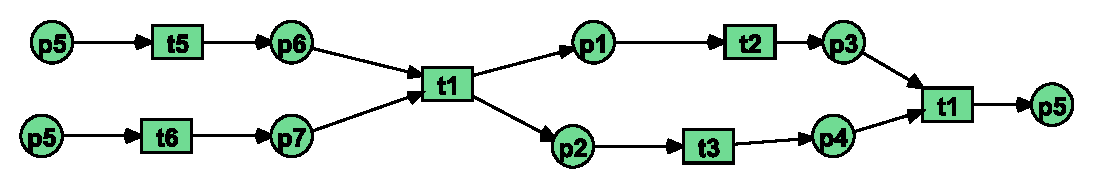
\includegraphics[scale=0.75]{Teilaufgaben/03-2.pdf}

\subsection*{3.}
Begründung für 1 gibt sich aus Konstruktion, da jeder Pfad einzeln beschrieben wurde.\\
zu 2.:\\
Auch die Mengen bezeichnen die einzelnen Pfade im Automaten
$\{d\} \cup \{ada\}\cup \{(ab)^n\}$ Beschreibt die "{}Sonderfälle"{}\\
\\
$ \{(ab)^md(ba)^m|m\leq n\ m\in\mathbb{N}\}$ Beschreibt dabei alle Pfade, die vor dem d auf b enden (also alle diejenigen, mit einer graden Anzahl von Buchstaben vor dem d)\\
\\
$ \cup \{a(ab)^mda(ba)^m|m< n\ m\in\mathbb{N}\}$ Beschreibt dabei alle Pfade, die vor dem d auf b enden (also alle diejenigen, mit einer ungraden Anzahl von Buchstaben vor dem d)\\
\subsection*{4.}
Offensichtlicherweise ist $L(A_n)$ Regulär, da der endliche DFA $A_n$ diese Sprache Akzeptiert.


\subsection*{4.}
sie sind auch nicht bisimilar, beispielsweise ist in $t_3$ die  (Aktions-)Folge babbc möglich, in $t_4$ jedoch nicht 

%\subsection*{5.}
%Wir setzen das Kantengewicht der kante von $p_2$ nach $t_4$ auf 1\\
Unsere Lösung ist in allen Fällen richtig, da die Anzahl der Marken immer gleich bleibt, diese marken können nur im Netz "{}herumwandern"{}.\\
\\
Unser Neues Netz ist außerdem Lebendig und (2-)beschränkt\\
\\
Alternativ könnte man ach eine Marke z.B. die aus $p_2$ entfernen, da es dann nur noch eine Marke im oberen Kreis gibt, kann $t_4$ niemals schalten. (Man könnte auch Alle Marken entfernen und hätte dann ein totes reversiebles netz)

%
%\subsection*{6.}
%Wir setzen das Kantengewicht der kante von $p_2$ nach $t_4$ auf 1\\
\begin{tikzpicture}[->,>=stealth',shorten >=1pt,auto,node distance=2.8cm,
                    semithick]
  \tikzstyle{every state}=[fill=none,draw=none,text=black]

  \node[state] (020)            				{$\begin{pmatrix} 0 \\2\\0 \end{pmatrix}$};
  \node[state] (110) [ above of=020]    		{$\begin{pmatrix} 1 \\1\\0 \end{pmatrix}$};  
  \node[state] (200) [ right of=110]         	{$\begin{pmatrix} 2 \\0\\0 \end{pmatrix}$};
  \node[state] (101) [ left of=020]        	{$\begin{pmatrix} 1 \\0\\1 \end{pmatrix}$};  
  \node[state] (011) [ below of=020]           	{$\begin{pmatrix} 0 \\1\\1 \end{pmatrix}$};
  \node[state] (002) [ right of=011]  		   	{$\begin{pmatrix} 0 \\0\\2 \end{pmatrix}$};
   

 

  \path (110) edge [bend left]         node {$t_2$} (200)
 		(110) edge [bend left]         node {$t_1$} (020)
 		(110) edge          node {$t_4$} (101)
		
 		(200) edge [bend left]         node {$t_1$} (110)

		(101) edge          node {$t_1$} (011)
		(101) edge [bend left]         node {$t_3$} (110)
 		
		(020) edge         node {$t_2$} (110)
 		(020) edge [bend left]         node {$t_4$} (011)
 		
		(011) edge [bend left]         node {$t_2$} (101)
		(011) edge         node {$t_3$} (020)
		(011) edge [bend left]         node {$t_4$} (002) 
		
		(002) edge [bend left]         node {$t_3$} (011)		
	
		;
        

\end{tikzpicture}



\pagebreak

\section*{\blattNr .4}

\subsection*{1.}

Ein Workflow-Netz $\mathcal{N}$ ist genau dann Korrekt, wenn sein Abschluss Lebendig und Beschränkt ist.\\
Dies Bedeutet, dass man Auch ein Netz $\mathcal{N}'$ alalysieren kann, dass aus $\mathcal{N}$ hervorgeht, wobei diese Eigenschaften erhalten bleiben.
%
\subsection*{2.}
%%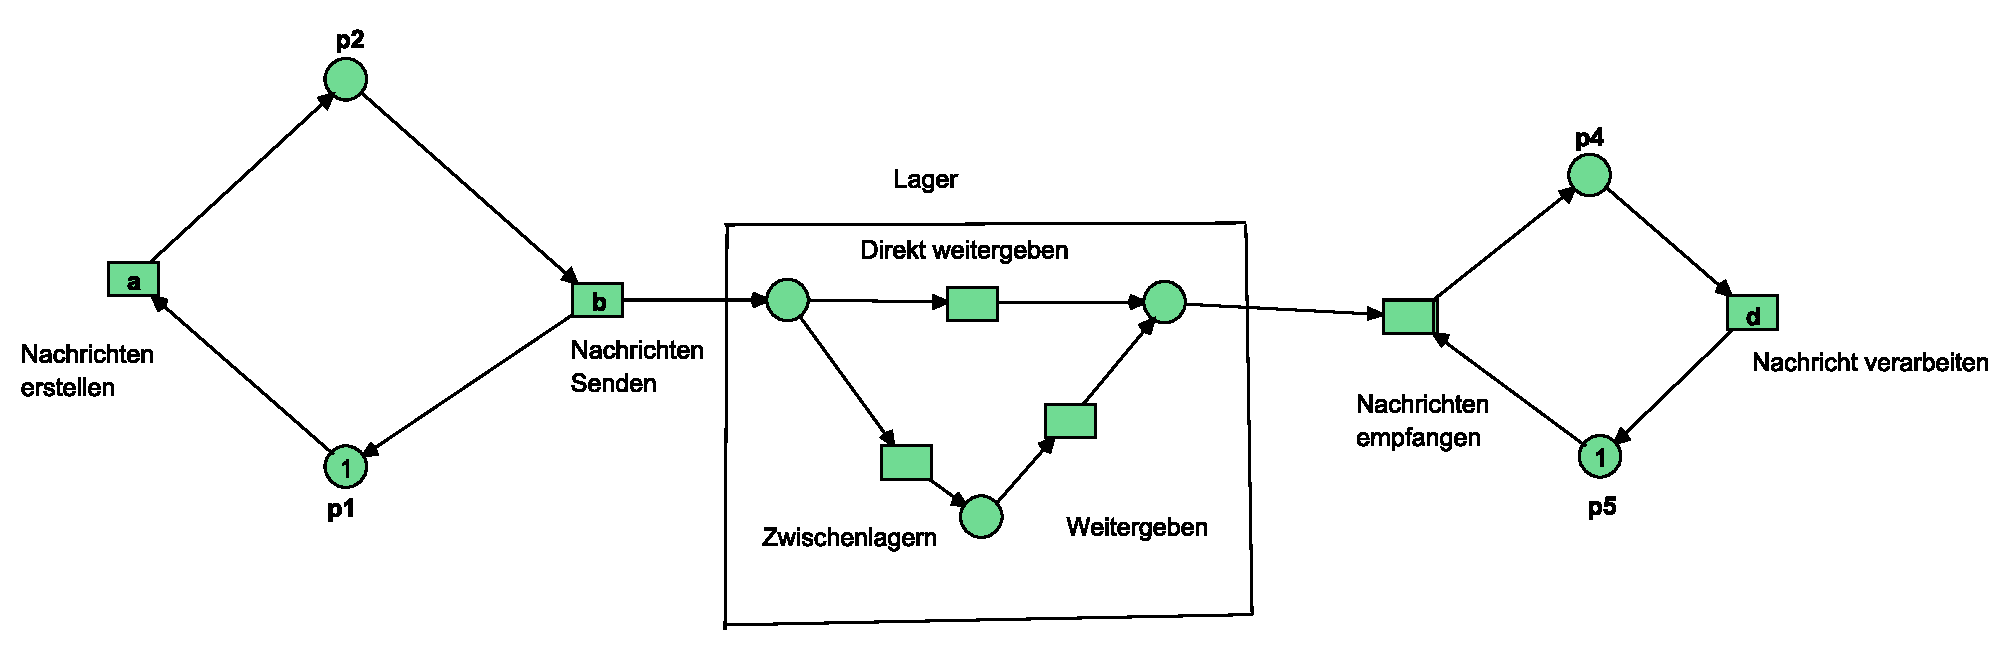
\includegraphics[scale=0.5]{Teilaufgaben/Aufgabe2.pdf}
\subsubsection*{(a)}

\[\Box(\neg Battery\Rightarrow\neg On)\]
true
\subsubsection*{(b)}
\[\Box\diamond On\]
false bei $\pi= c_0c_1c_2c_3(c_4)^\omega$
\subsubsection*{(c)}
\[\Box ( \circ Error \Rightarrow Acrive)\]
false bei $\pi= c_0c_1c_2c_3(c_4)^\omega$
(Das gerät befindet sich am ende immer nur noch im Fehler und war vorher auch im fehler)
\subsubsection*{(d)}
\[\Box (On\vee Error \vee \circ On)\]
true
 	
%%
%\subsection*{3.}
% 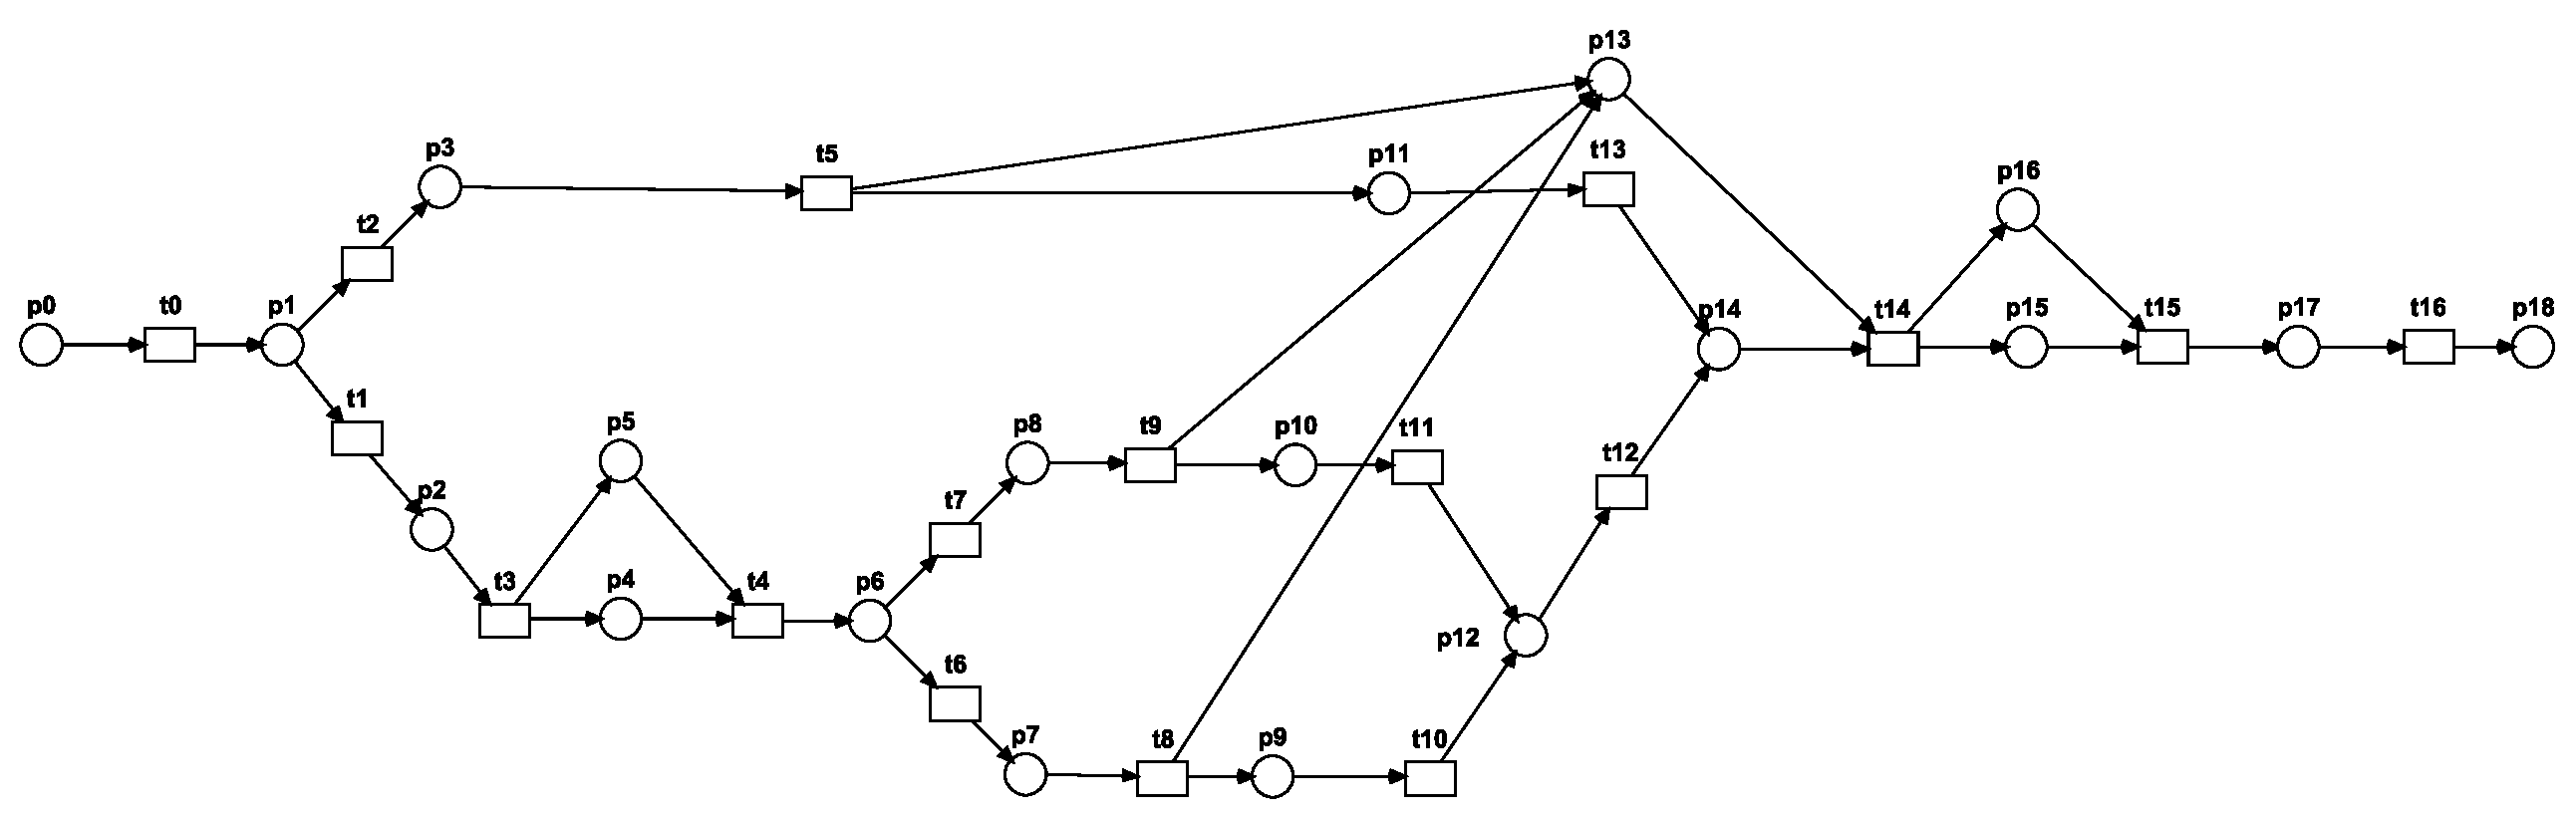
\includegraphics[scale=0.3]{Teilaufgaben/vorlage.pdf}\\
 Anwenden d	er Regel T-Seq:\\
 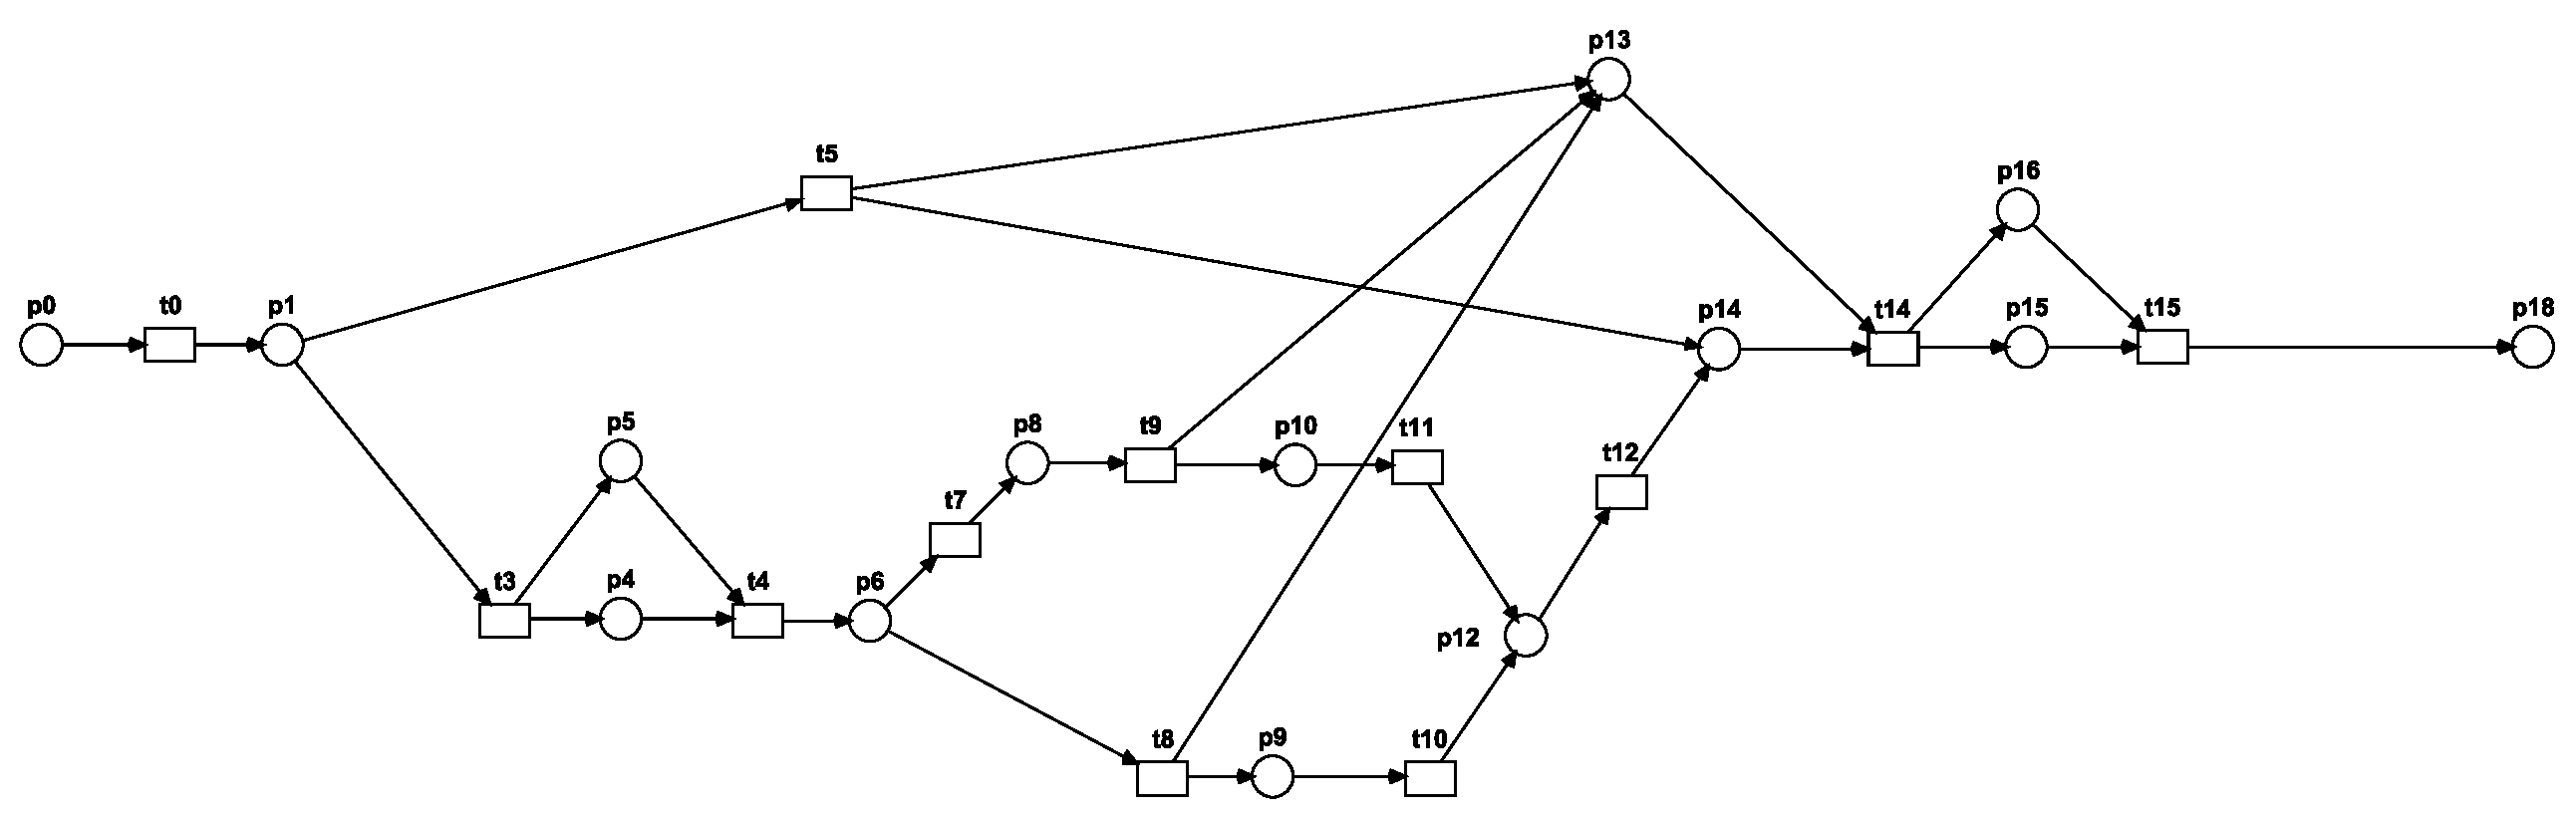
\includegraphics[scale=0.3]{Teilaufgaben/tseq1.pdf}\\
 
  Anwenden der Regel Par:\\
 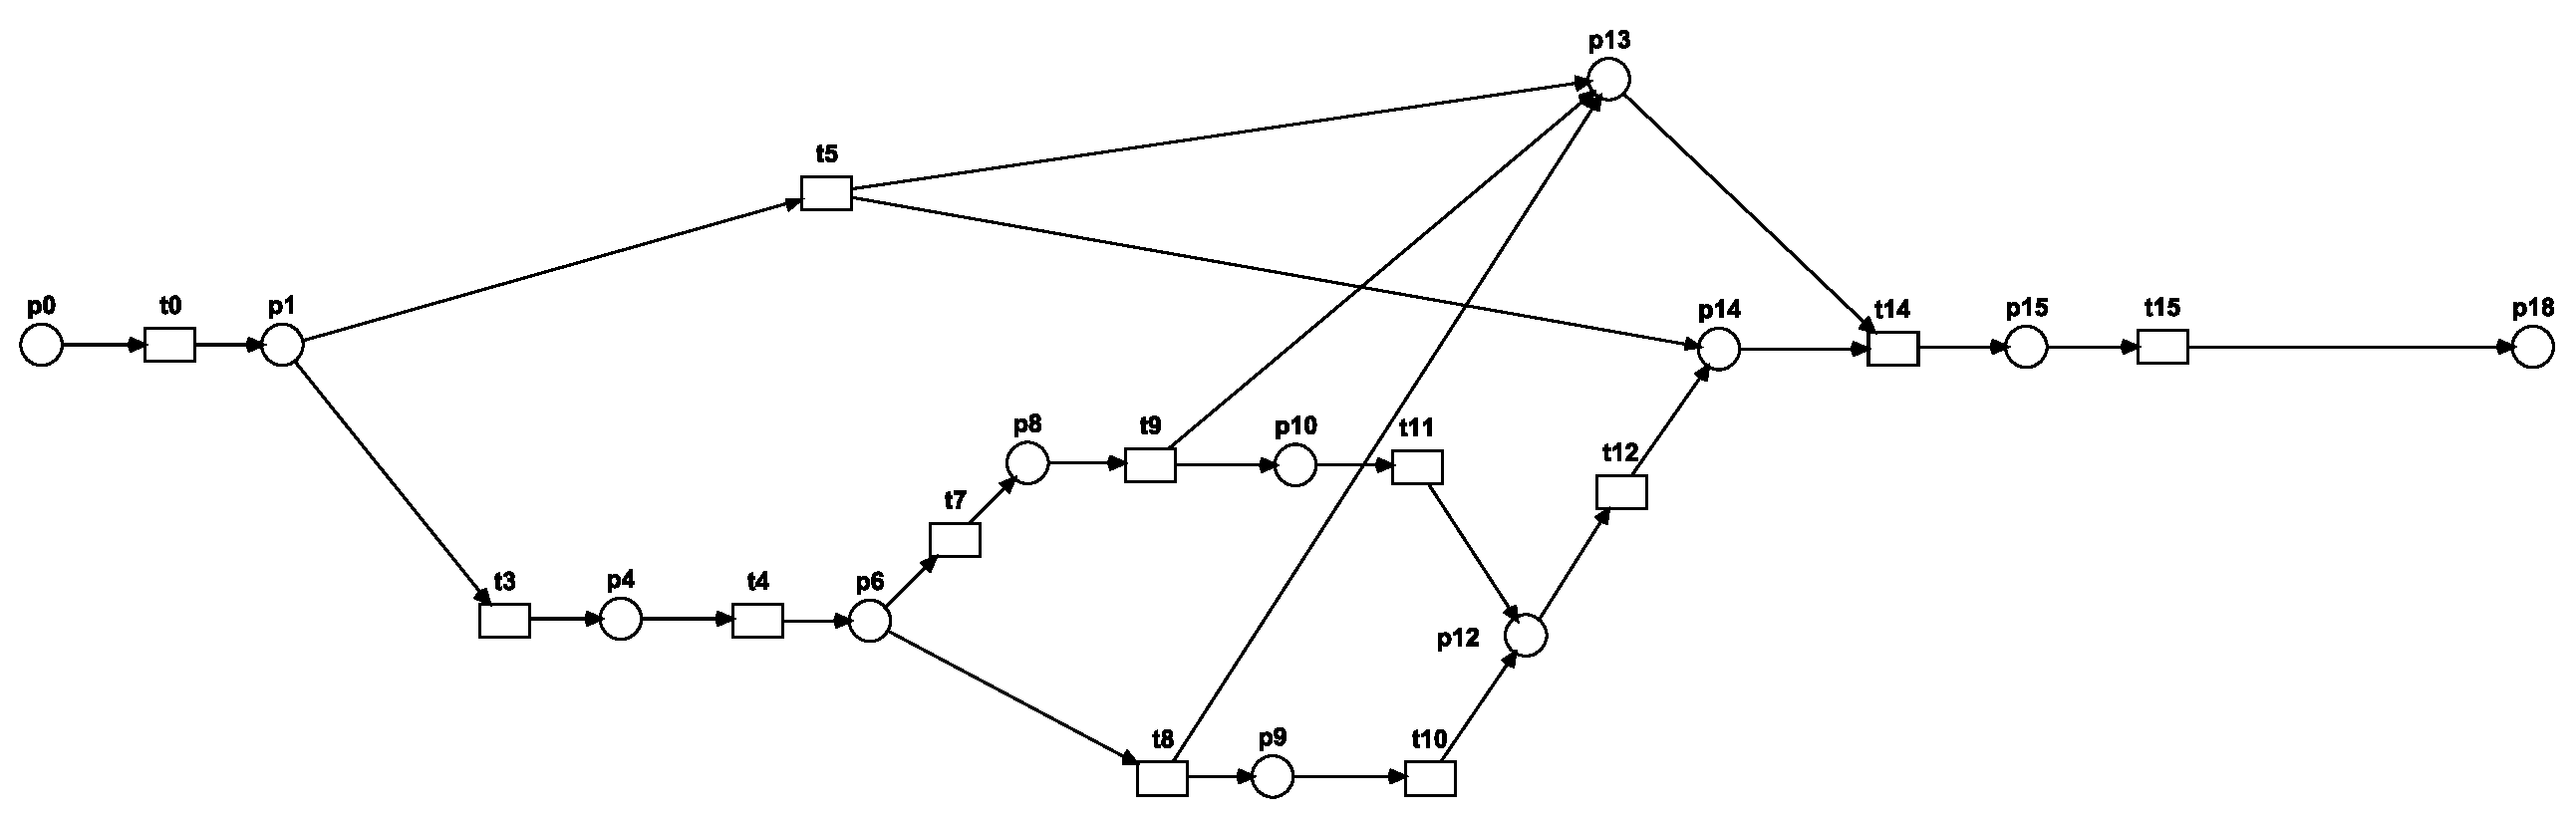
\includegraphics[scale=0.3]{Teilaufgaben/par1.pdf}\\
 
   Anwenden der Regel P-Seq:\\
 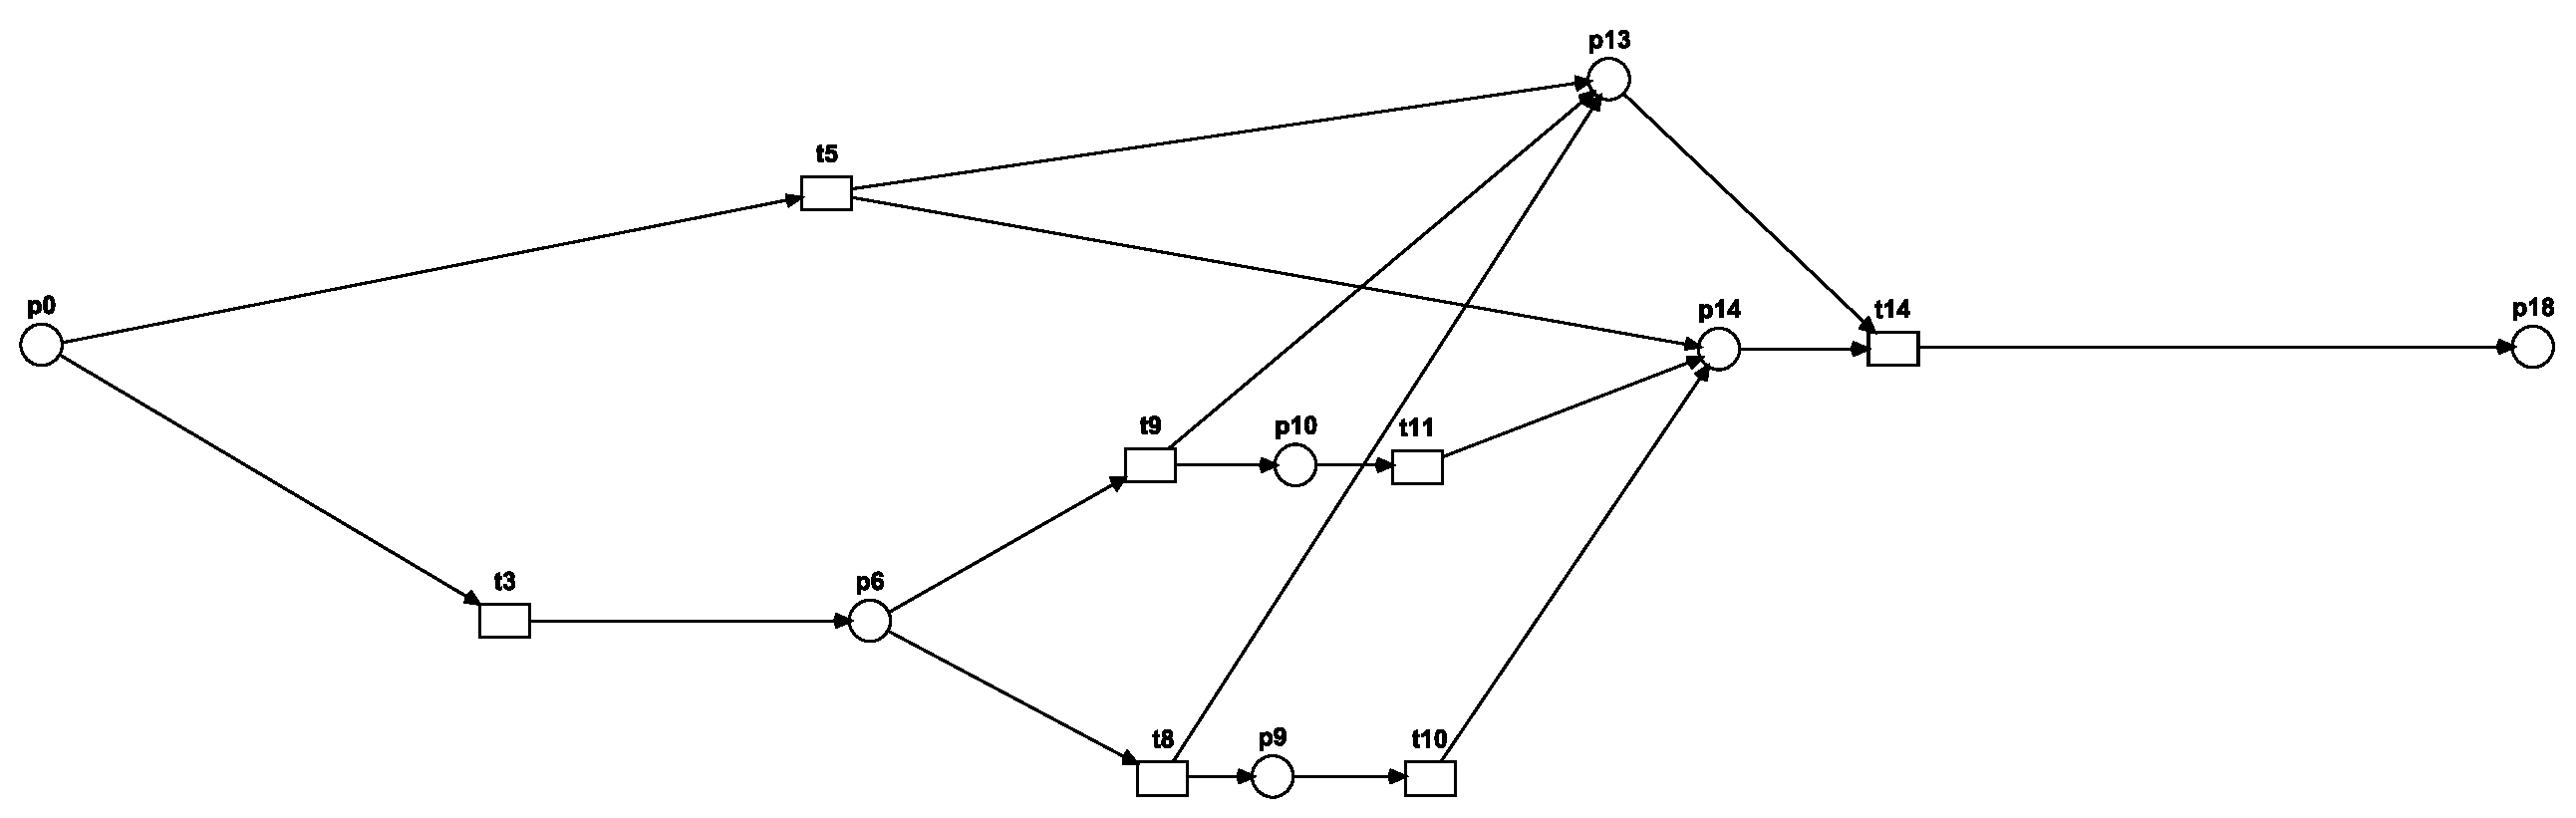
\includegraphics[scale=0.3]{Teilaufgaben/pseq1.pdf}\\
 
    Anwenden der Regel P-Seq:\\
 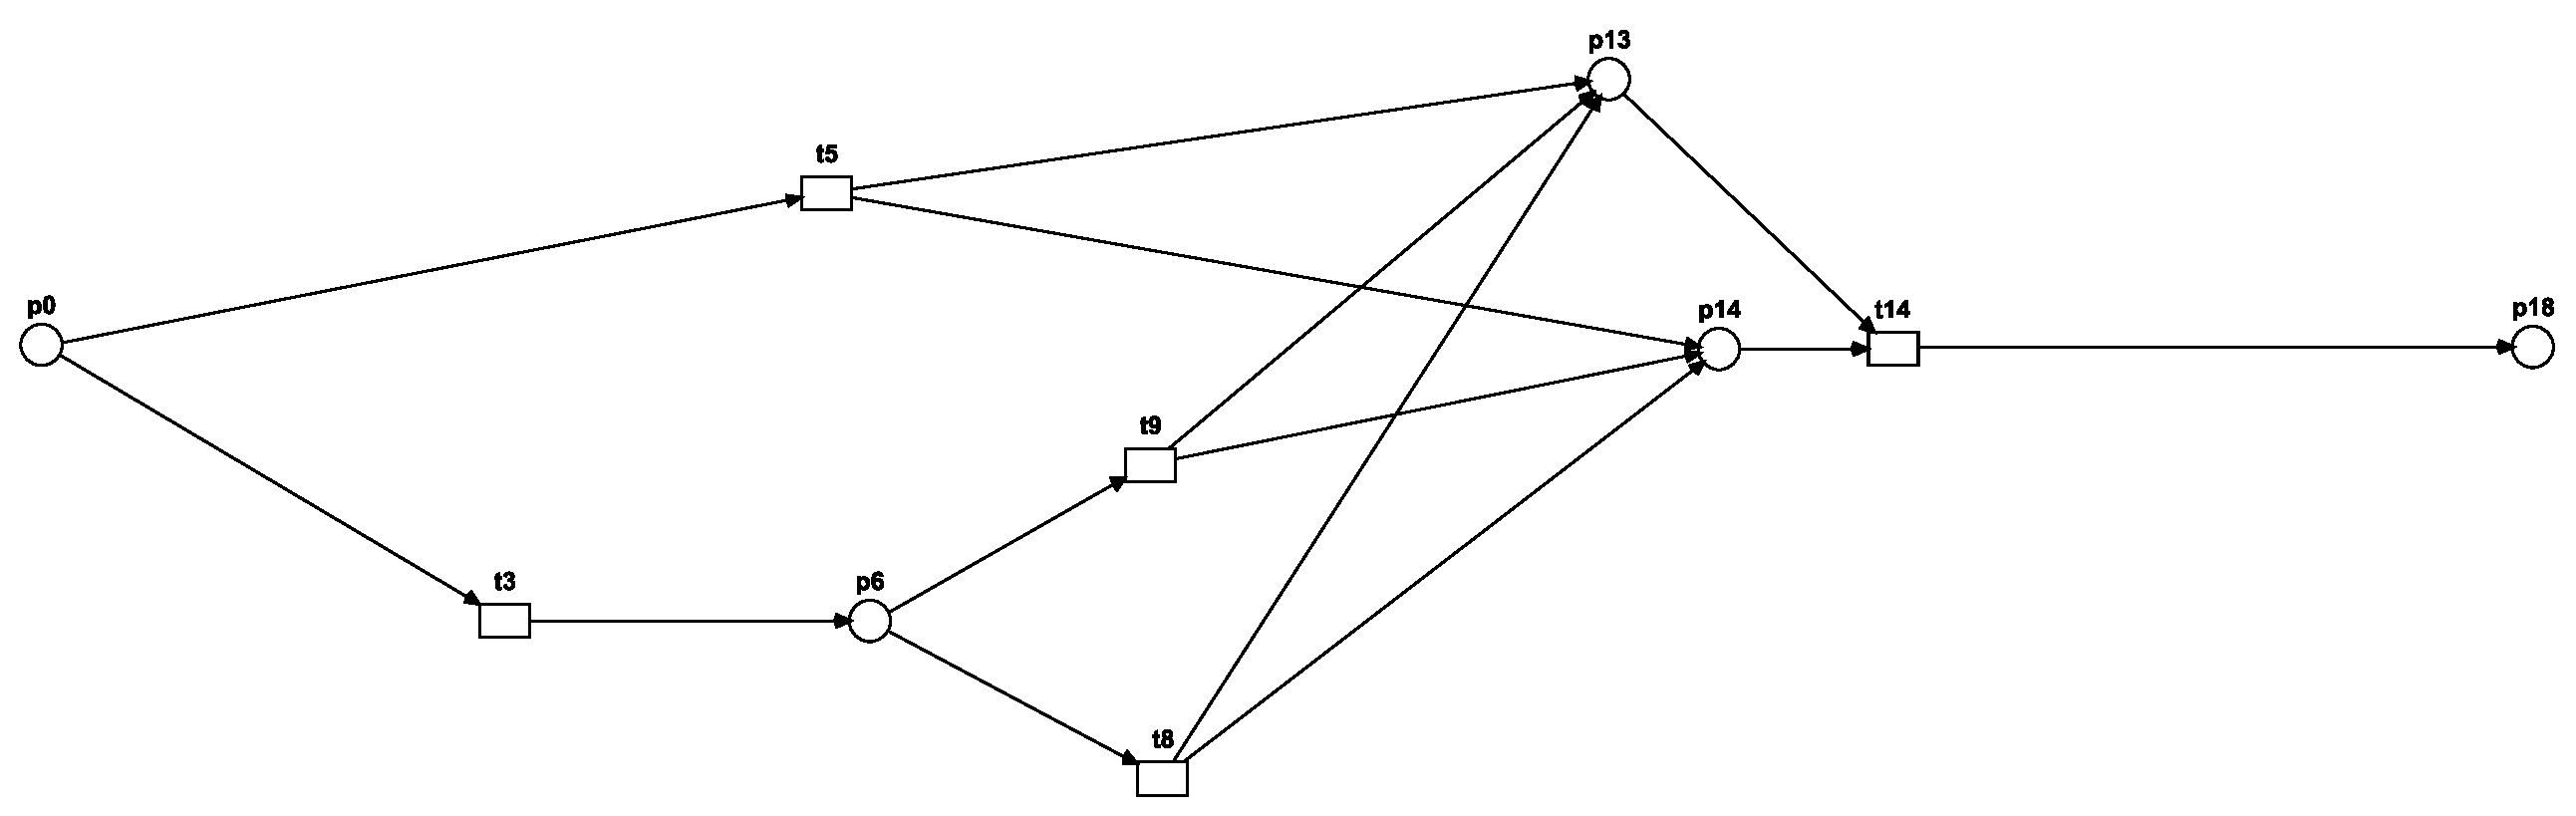
\includegraphics[scale=0.3]{Teilaufgaben/pseq2.pdf}\\
 
     Anwenden der Regel Par:\\
 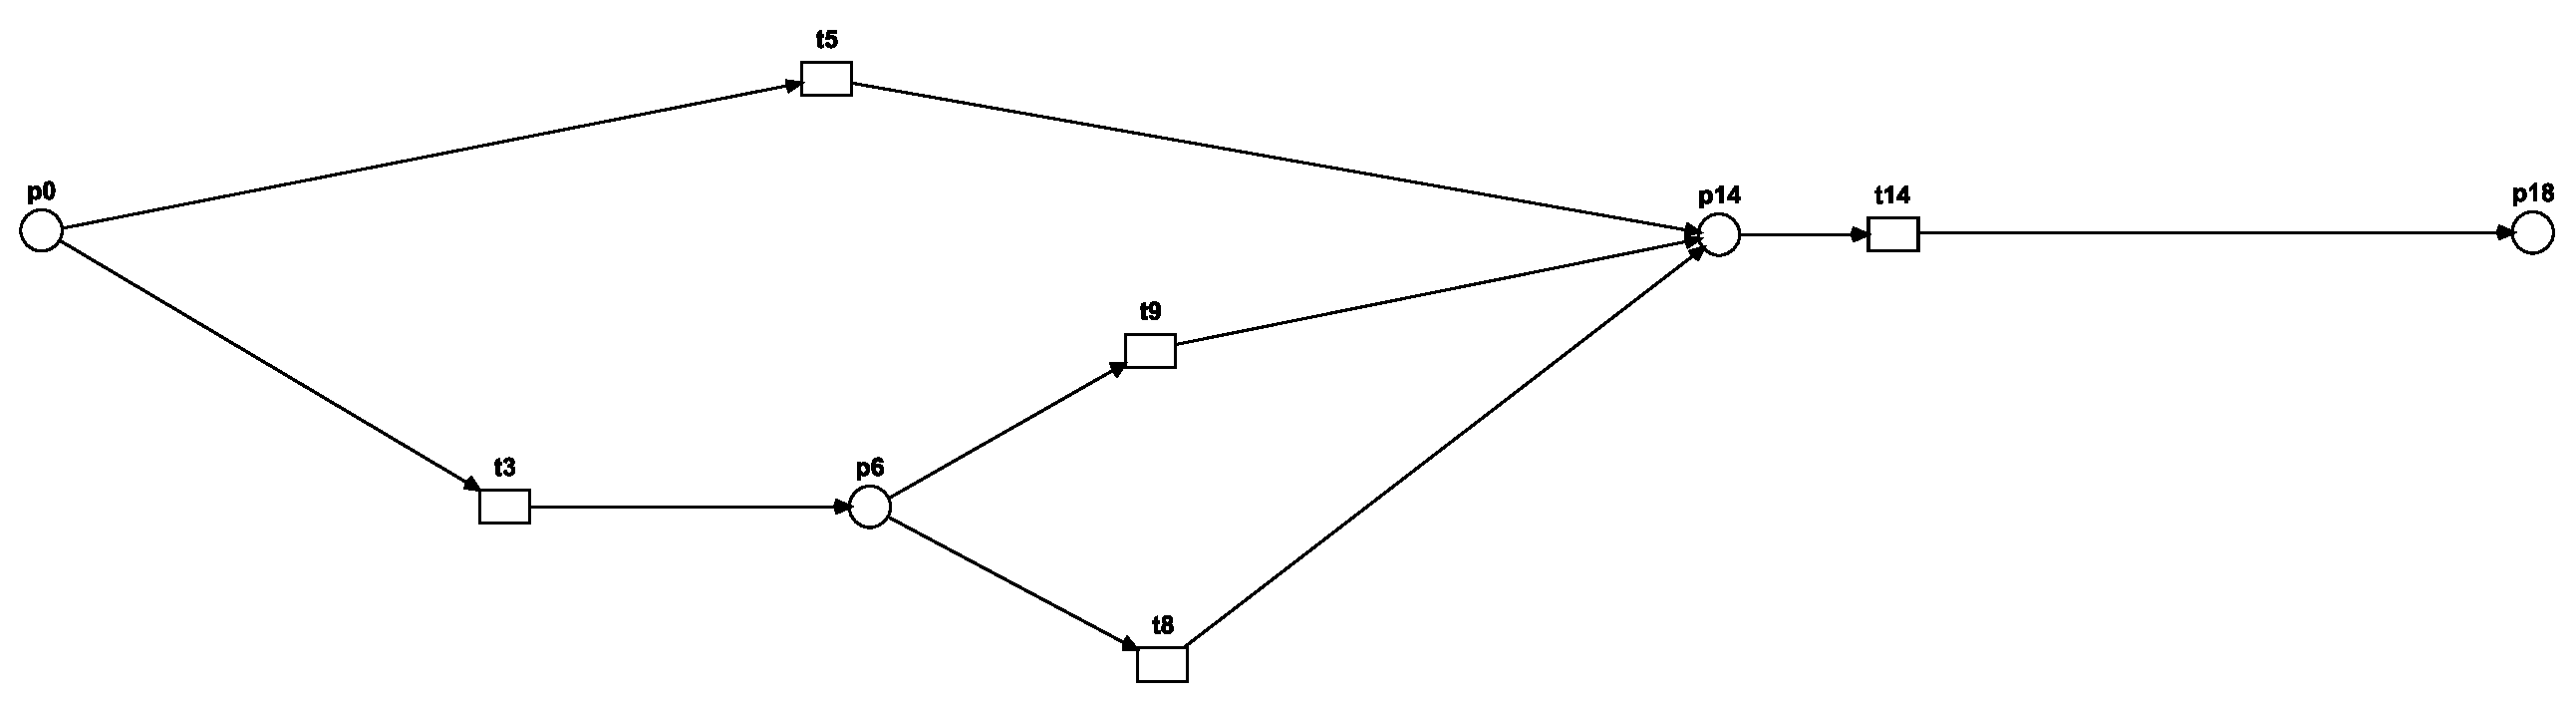
\includegraphics[scale=0.3]{Teilaufgaben/par2.pdf}\\
 
     Anwenden der Regel P-Seq:\\
 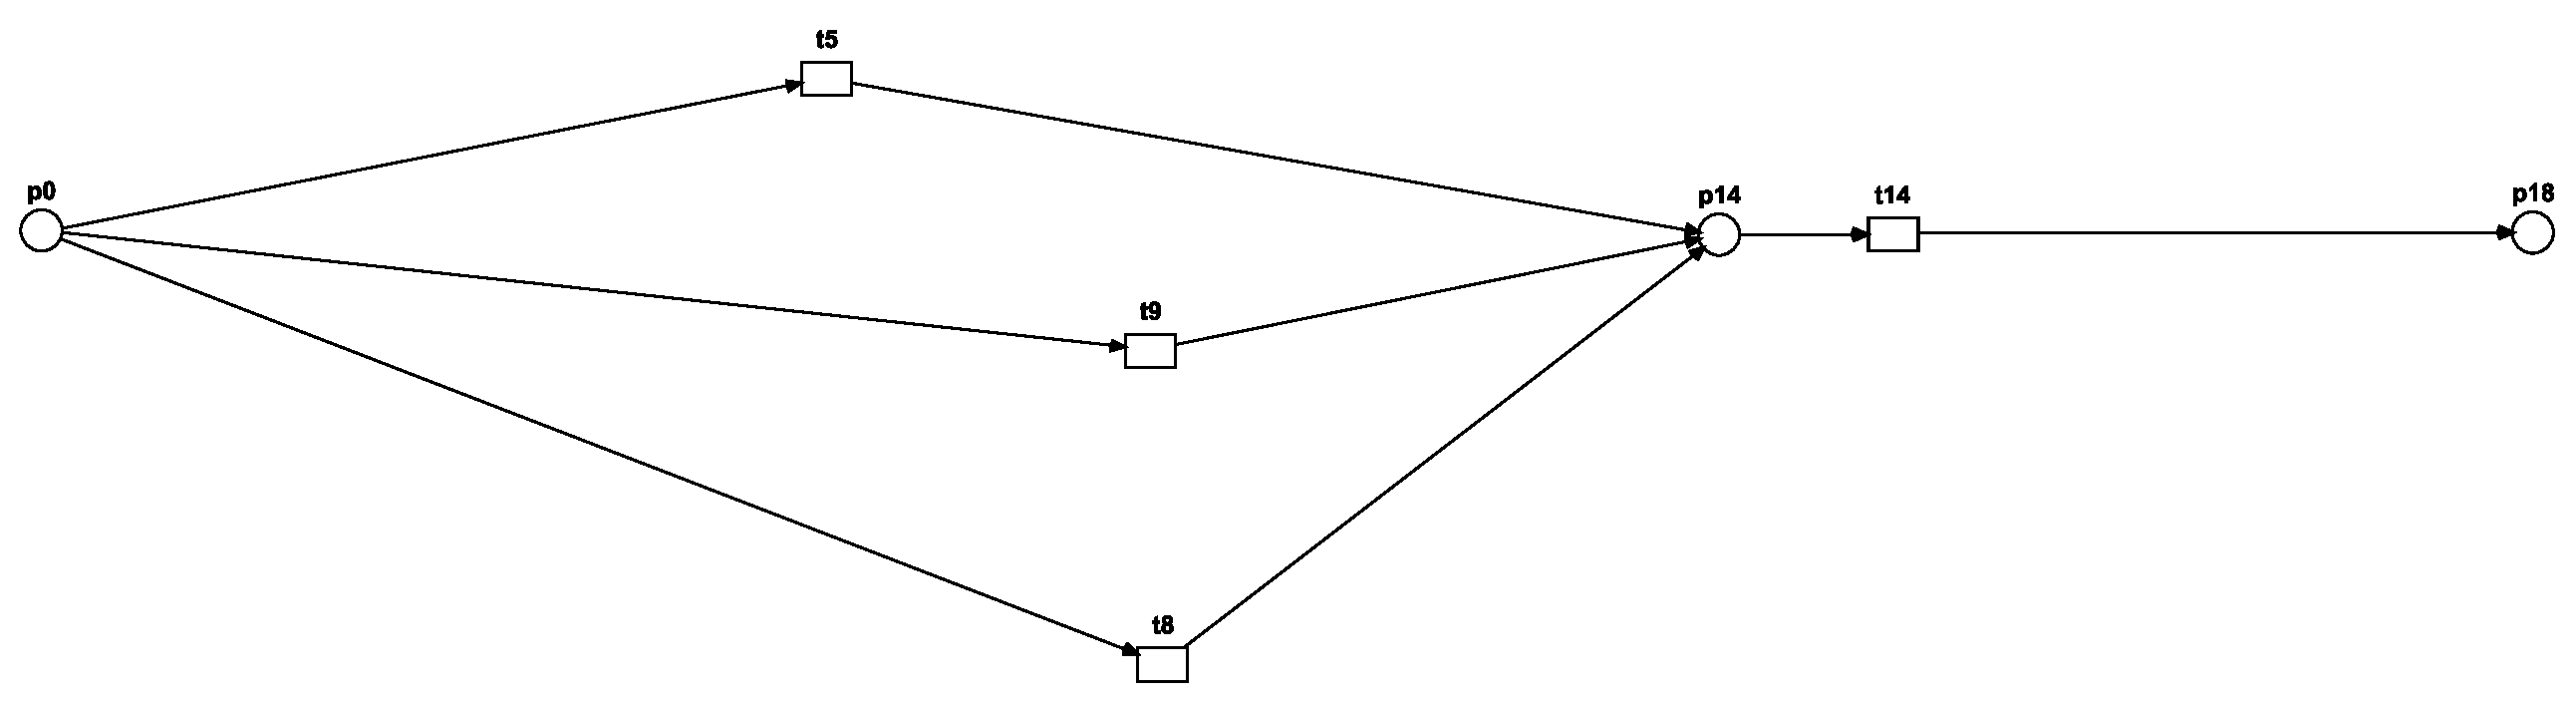
\includegraphics[scale=0.3]{Teilaufgaben/pseq3.pdf}\\
 
      Anwenden der Regel Alt:\\
 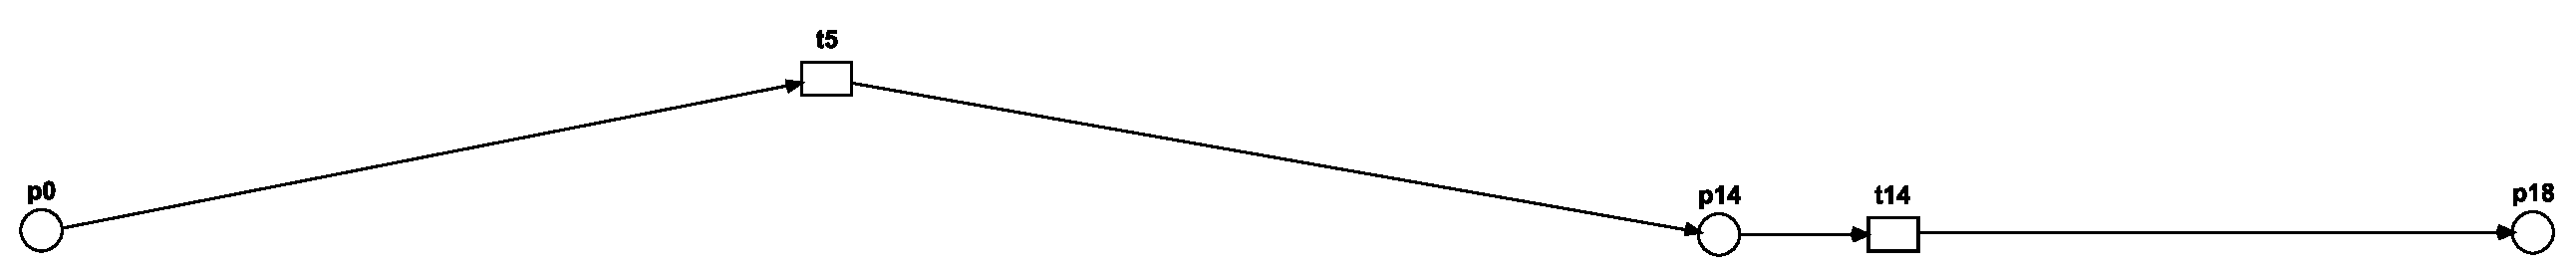
\includegraphics[scale=0.3]{Teilaufgaben/alt1.pdf}\\
 
       Anwenden der Regel T-Seq:\\
 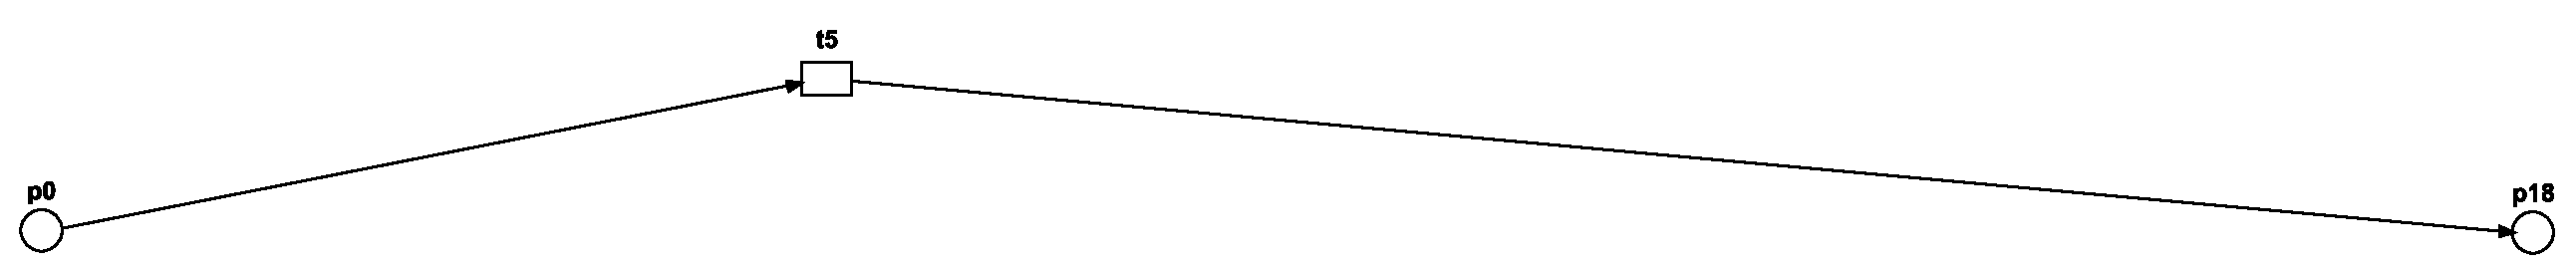
\includegraphics[scale=0.3]{Teilaufgaben/tseq2.pdf}\\
 
 Angekommen Beim trivialen Korrekten Netz, Das Ursprünglihce Netz muss daher auch Korrekt sein.
%%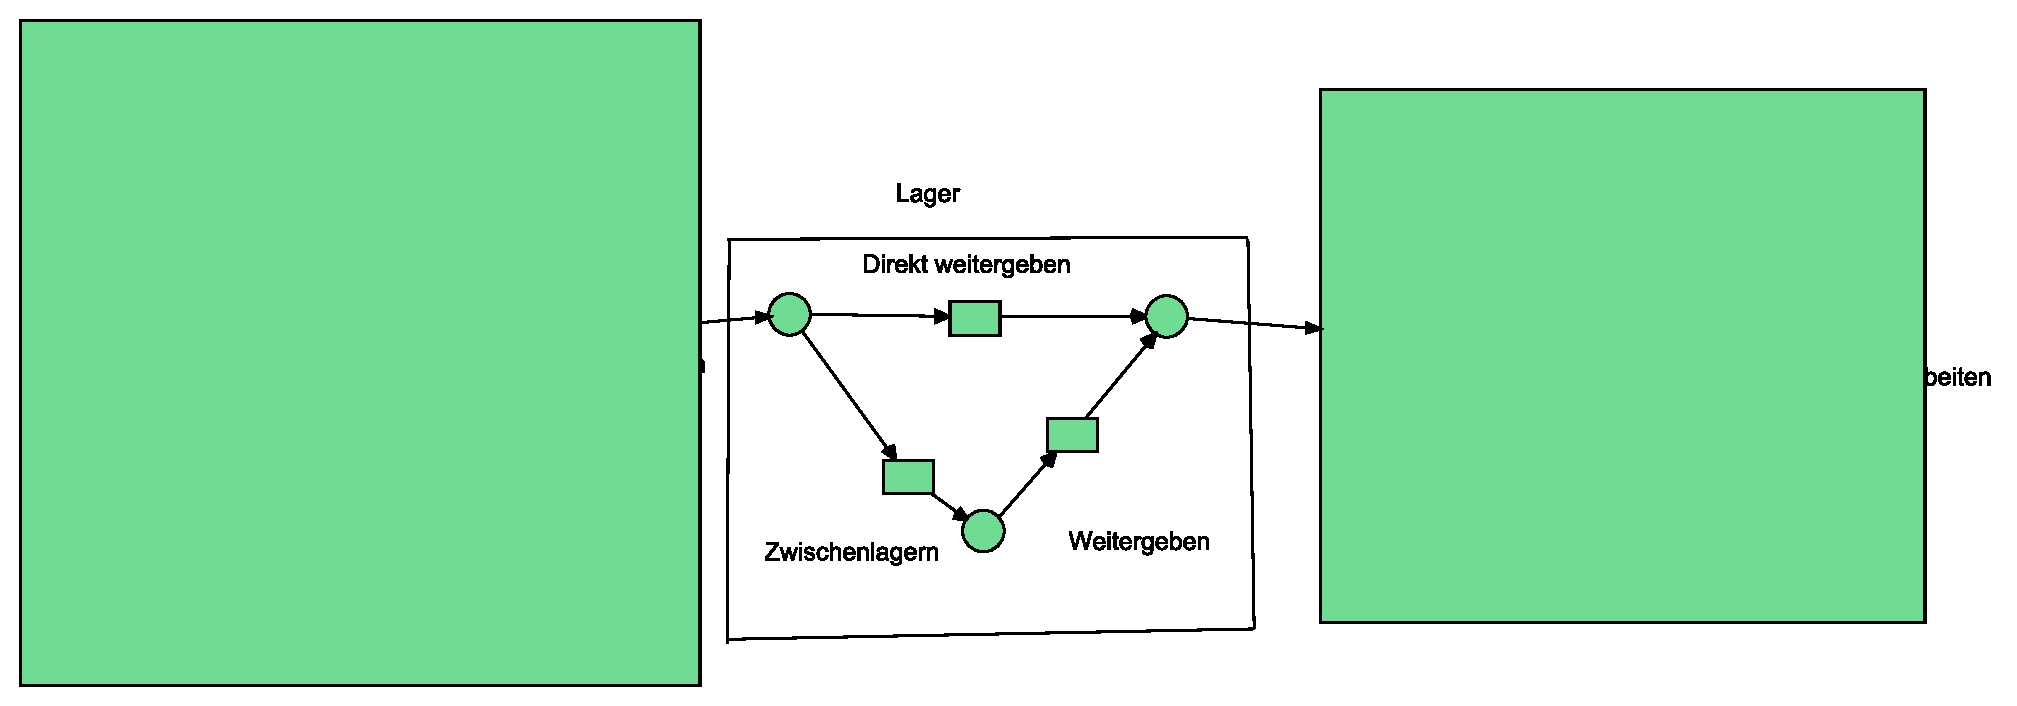
\includegraphics[scale=0.5]{Teilaufgaben/Aufgabe3.pdf}
%
%\subsection*{4.}
%\usetikzlibrary{automata,arrows}


Als erstes müssen wir den DFA A in A$rev$, also den DFA der all jene Eingaben akzeptiert die das Teilwort $deer$ enthalten.

Hierfür werden alle Kanten umgedreht und Start- und Endzustand vertauscht.

So wird

\begin{figure}[ht]
\centering
\begin{tikzpicture}[->,>=stealth',shorten >=1pt,auto,node distance=2.5 cm, scale = 1, transform shape]

%\tikzstyle{every state}=[fill=white,draw=black,text=black]

%Erstelle 5 Zustände

\node[initial,state]	(A)					{$q_0$};
\node[state]			(B)	[right of =A]	{$q_1$};
\node[state]			(C)	[right of =B]	{$q_2$};
\node[state]			(D)	[right of =C]	{$q_3$};
\node[state,accepting]	(E)	[right of =D]	{$q_4$};

%Erstelle Übergänge
\path	(A)	edge					node	{r} 	(B)
			edge	[loop above]	node	{d,e}	(A)
		(B)	edge					node	{e}		(C)
			edge	[loop above]	node	{r}		(B)
			edge	[bend left]		node	{d}		(A)
		(C) edge					node	{e}		(D)
			edge	[bend left]		node	{r}		(B)
			edge	[bend left]		node	{d}		(A)
		(D) edge					node	{d}		(E)
			edge	[bend right]	node	{r}		(B)
			edge	[bend left]		node	{e}		(A)
		(E) edge	[loop above]	node	{r,e,d}	(E);


\end{tikzpicture}
\caption{Der Ursprüngliche DFA A}
\end{figure}

in 

\begin{figure}[ht]
\centering
\begin{tikzpicture}[->,shorten >=1pt,auto,node distance=2.5 cm, scale = 1, transform shape]

%\tikzstyle{every state}=[fill=white,draw=black,text=black]

%Erstelle 5 Zustände

\node[state,initial]	(E)					{$q_4$};
\node[state]			(D)	[right of =E]	{$q_3$};
\node[state]			(C)	[right of =D]	{$q_2$};
\node[state]			(B)	[right of =C]	{$q_1$};
\node[state,accepting]	(A)	[right of =B]	{$q_0$};

%Erstelle Übergänge
\path	(A)	edge	[loop above]	node	{d,e}	(A)
			edge	[bend left]		node	{d}		(B)
			edge	[bend left]		node	{d}		(C)
			edge	[bend left]		node	{e}		(D)
		(B)	edge					node	{r}		(A)
			edge	[loop above]	node	{r}		(B)
			edge	[bend right]	node	{r}		(D)
			edge	[bend left]		node	{r}		(C)
		(C) edge					node	{e}		(B)
		(D) edge					node	{e}		(C)
		(E) edge					node	{d}		(D)
			edge	[loop above]	node	{r,e,d} (E);

\end{tikzpicture}
\caption{Der NFA A rev}
\end{figure}

umgewandelt.

Anschließend benutzen wir die Potenzautomatenkonstruktion um den Automaten in folgenden zu überführen:

\begin{figure}[ht]
\centering
\begin{tikzpicture}[->,shorten >=1pt,auto,node distance=2.5 cm, scale = 1, transform shape]

%\tikzstyle{every state}=[fill=white,draw=black,text=black]

%Erstelle 5 Zustände

\node[state,initial]	(E)			{$\{q_4\}$};
\node[state]		(ED)	[right of =E]	{$\{q_4,q_3\}$};
\node[state]		(C)	[right of =D]	{$\{q_2\}$};
\node[state]		(B)	[right of =C]	{$\{q_1\}$};
\node[state,accepting]	(A)	[right of =B]	{$\{q_0\}$};
\node[state,accepting]	(ABCD)	[above of =B]	{$\{q_0,q_1,q_2,q_3\}$};



%Erstelle Übergänge
\path	(E) 	edge	[loop above]	node 	{r,e}	(E)
		edge	[bend left]	node	{d}		(ED)
	(ED)	edge	[bend left]	node	{e}		(C)
		edge	[bend left]	node	{r}		(E)
		edge	[loop below]	node	{d}	(D)
	(C)	edge	[bend left]	node	{r,d}	(ED)
		edge			node	{e}		(B)
	(B)	edge	[bend left]	node	{e,d}	(B)
		edge	[bend right]	node	{r}		(ABCD);
\end{tikzpicture}
\caption{Der Potenzautomat A rev}
\end{figure}


Damit haben wir den Algorithmus abgearbeitet und einen Automaten erzeugt der das gewünschte leistet (wie in 5. gezeigt wird).
%%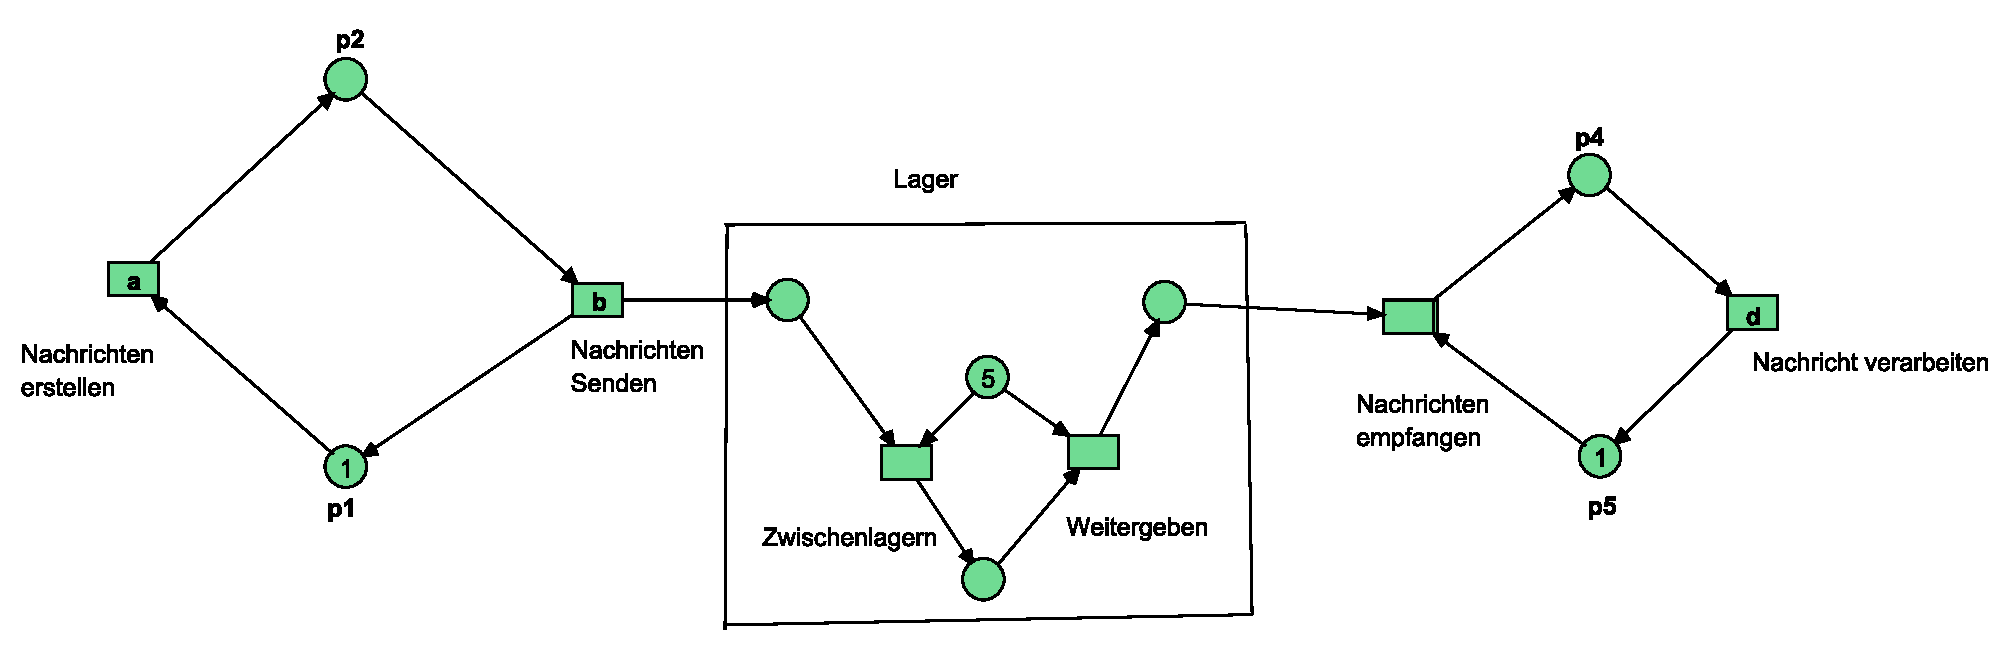
\includegraphics[scale=0.5]{Teilaufgaben/Aufgabe4.pdf}
%
%\subsection*{5.}
%%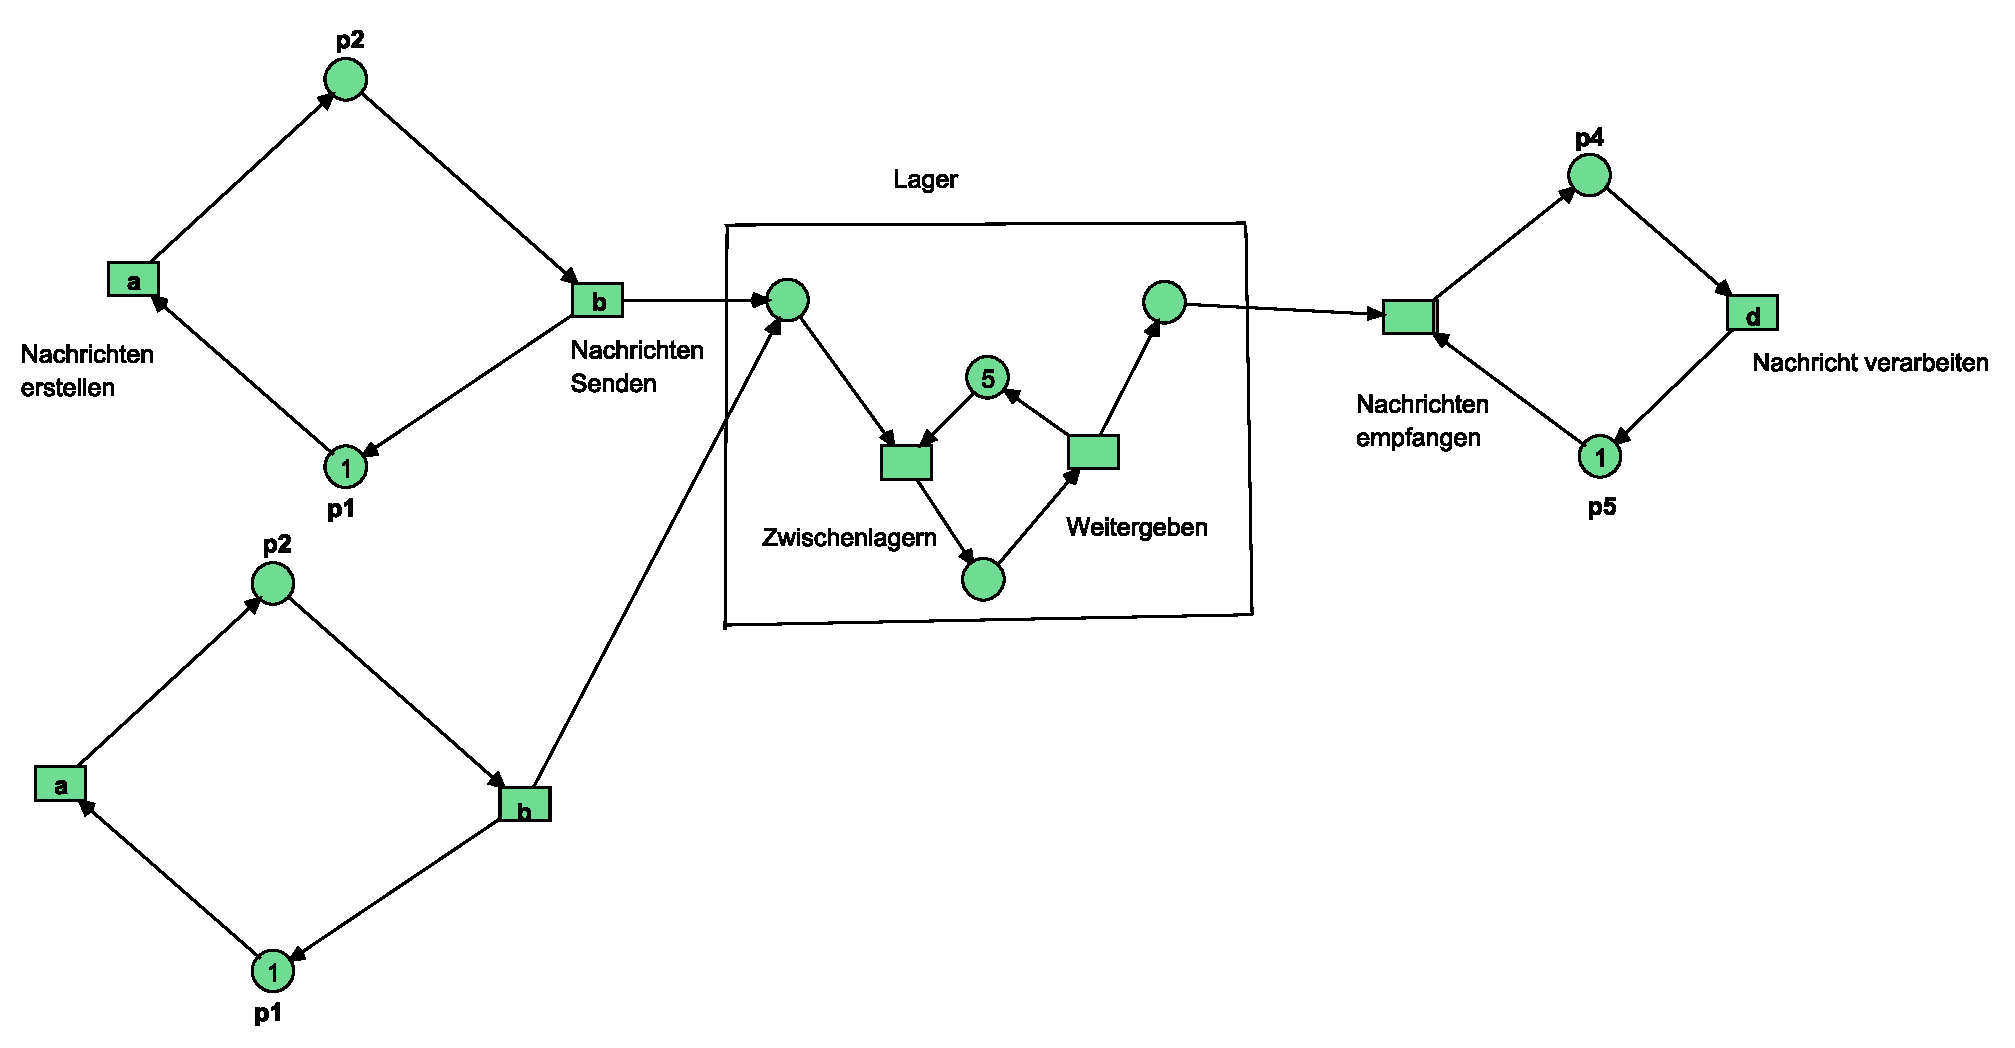
\includegraphics[scale=0.5]{Teilaufgaben/Aufgabe5.pdf}
%siehe 1.
%%
%\subsection*{8.}
%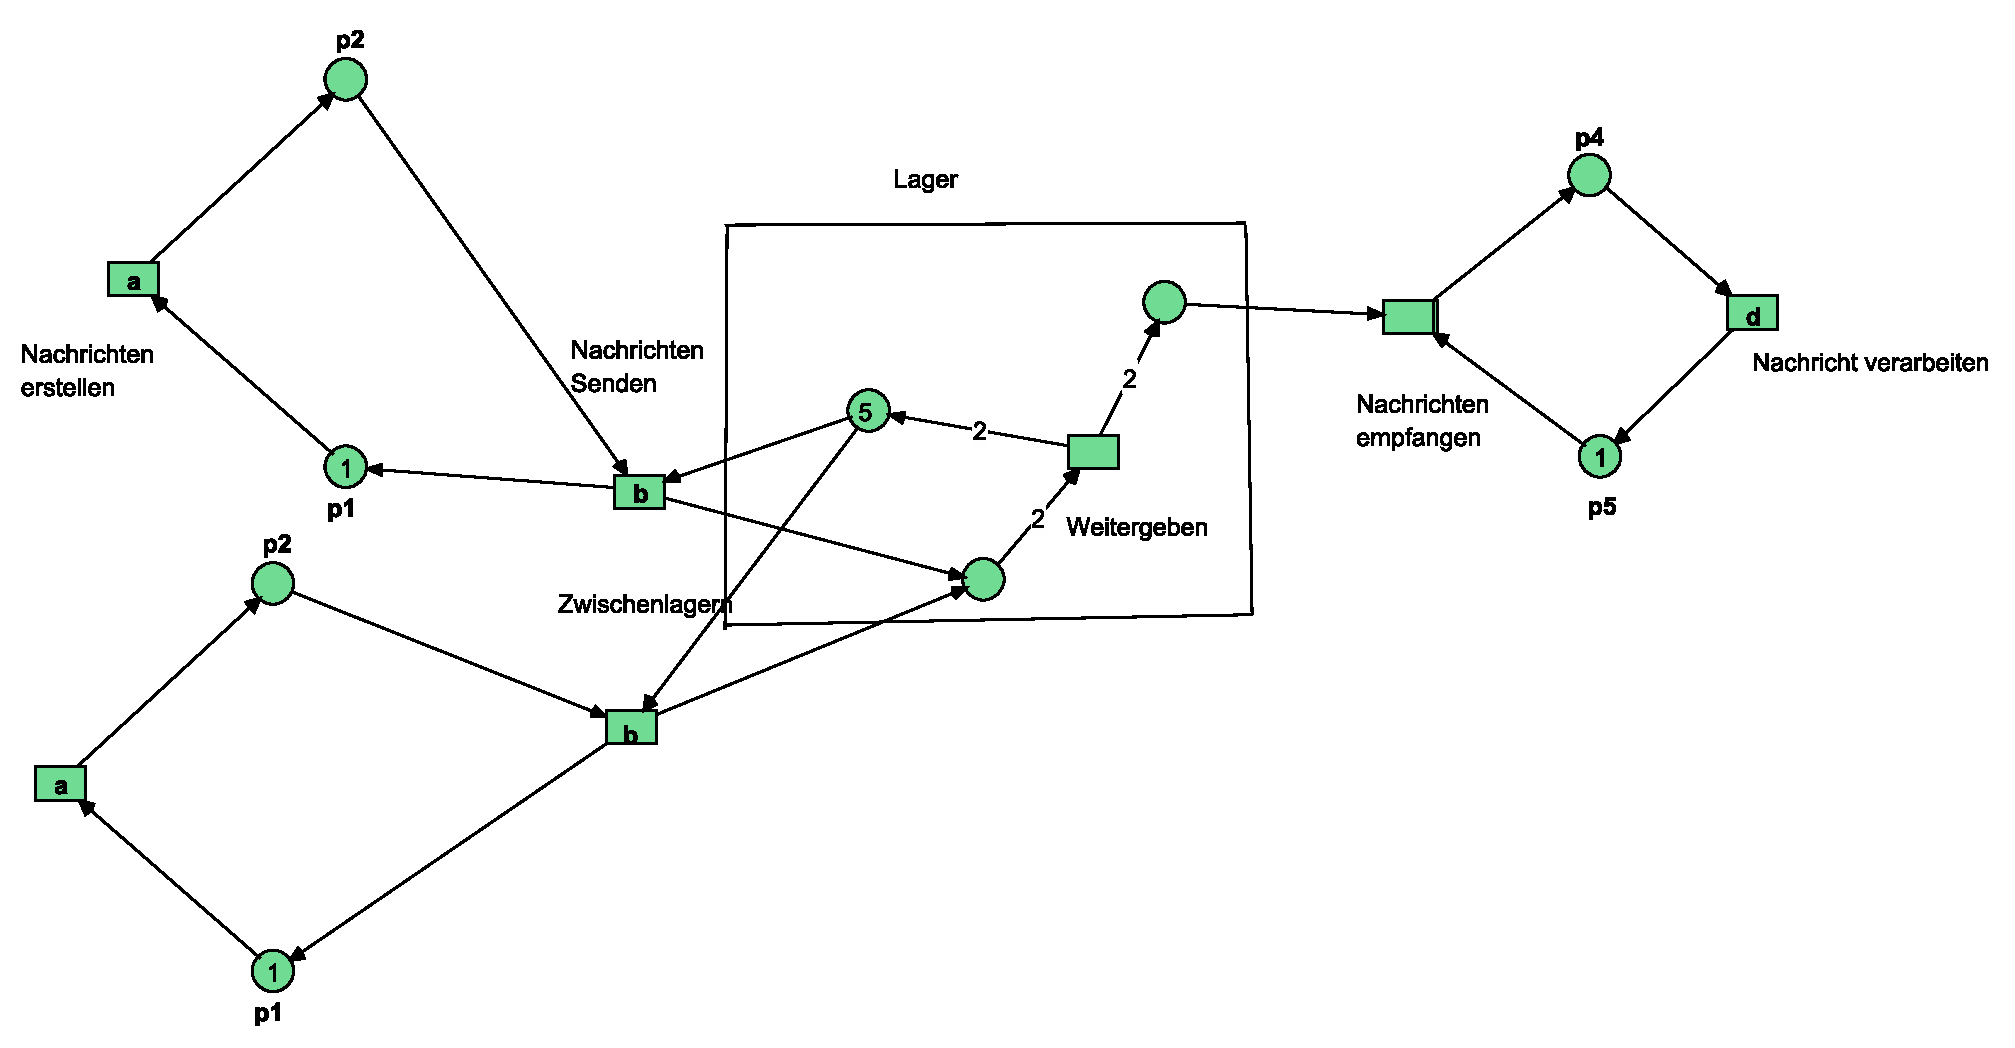
\includegraphics[scale=0.5]{Teilaufgaben/Aufgabe6.pdf}
%Angenommen das Netz Sei Vor dem Anwenden Der regel Beschränkt, so ist dies Auch nach dem Anwenden Der Regel der Fall, Das Entfernen einer Transition, kann die Beschränktheit nicht zerstören.\\
Angenommen das Netz sie Vor dem anwenden Der Regel unbeschränkt, so ist es dies auch nach dem Anwenden Der Regel, Da Jedes Auftreten von der Entfernten Transition in irgenteiner Schaltfolge durch die Weiterhin vorhandene Transition mit gleihcem vor und Nachbereich ersetzt werden kann, ohne die Auftretenden Markierungen zu ändern.

\end{document}
